\documentclass[onecolumn]{report}
\pdfpagewidth=8.5in
\pdfpageheight=11in


% Use the postscript times font!
\usepackage{ijcai19}
\usepackage{times}
\usepackage{soul}
\usepackage{url}
\usepackage[hidelinks]{hyperref}
\usepackage[utf8]{inputenc}
\usepackage[small]{caption}
\usepackage{graphicx}
\usepackage{amsmath}
\usepackage{booktabs}
\usepackage{multirow}
\usepackage{csquotes}
\newcommand\numberthis{\addtocounter{equation}{1}\tag{\theequation}}


\urlstyle{same}

\title{%
	Least absolute shrinkage and selection operator (LASSO) regresija s poudarkom na varinatah \emph{sampleLASSO} in \emph{geneLASSO} \\
	\ \\
	\large Zaključni projekt pri predmetu Strojno učenje}

\author{
	Maks Evgen Obelšer \\ 
	\ \\ 
	\large 64200409
}

\begin{document}

\maketitle

\section{Uvod}

Regresijska analiza je statističen proces ocenjevanja odnosa med odvisno spremenljivko in eno ali več neodvisnih spremenljivk. Najosnovnejša oblika ja linearna regresija, ki najde premico (ali bolj kompleksno linearno kombinacijo), ki se najbolj prilega opazovanim podatkom glede na specifični matematični kriterij. Recimo metoda navadnih najmanjših kvadratov izračuna premico (ali hiperravnino v primeru več neodvisnih spremenljivk), ki minimizira vsoto kvadratov razlik med podatki in to premico (ali hiperravnino). 

To omogoči raziskovalcu, da oceni pogojno pričakovano vrednost (ali populacijsko povprečje) odvisne spremenljivke glede na neodvisno spremenljivko (ali set neodvisnih spremenljivk). 

V statistiki in strojnem učenju je linearna regresija robustna in splošno zelo uporabljena metoda, za katero pa obstaja veliko specialnih variant, ki omogočajo boljše napovedi. Primer takih prilagoditev so posplošeni linearni modeli in hierarhična linearna regresija. 

\section{Least absolute shrinkage and selection operator (LASSO)}

Kot ime nakazuje, je LASSO regresija metoda, ki omogoči izbiro spremenljivk in regularizacijo modela z namenom izboljšave napovedne točnosti in interpretativnosti. Metoda je bila neodvisno razvita an geofizikalnem področju na podlagi prejšnjega dela z $\ell^1$ kaznijo za prileganje in kaznovanje koeficientov. Robert Tibshirani jo je leta 1996 neodvisno ponovno odkril in populariziral. Pred tem je bila splošno uporabljana metoda za izbiro kovariat postopna izbira, kjer postopno dodajamo kovariate v model in na ta način izberemo najprimernejšo kombinacijo. LASSO zelo dobro deluje, ko imamo nekaj kovariat, ki so zelo povezane z izidom med veliko kovariatami, ki niso. 

Metoda se veliko uporablja na področju visoko-dimenzionalnih podatkov, saj rešuje problem $n \ll p$, kjer je $n$ število opazovanj in $p$ število spremenljivk. Pri OLS regresiji naletimo na problem, da modelska matrika v tej situaciji nima polnega ranga, kar pa LASSO ne predpostavlja.

\section*{Definicija}

Imamo podatke $(x^i, y^i), \	 i = 1, 2, ..., N$, kjer so $x^i = (x_{i1}, ..., x_{ip})^T$ napovedne spremenljivke in $y_i$ odvisne spremenljivke, torej imamo podatke z $n$ opazovanji in $p$ napovednimi spremenljivkami. Kot pri navadnem regresijskem problemu, predpostavimo, da so opazovanja neodvisna in da so $y_i$ pogojno neodvisni od $x_{ij}$. Prav tako predpostavimo, da so $x_{ij}$ standardizirani, torej velja $\sum_{i = 1}^{N} x_{ij}/N = 0$ (povprečje po spremenljivkah je enako 0) in $\sum_{i = 1}^{N} x_{ij}^2/N = 1$ (standardni odklon je enotski in enak 1). 

Kjer je $\hat{\beta} = (\hat{\beta_1}, ..., \hat{\beta_p})^T$ je LASSO ocena parametrov $(\hat{\alpha}, \hat{\beta})$ enaka:

\begin{align*}
	(\hat{\alpha}, \hat{\beta}) = & \underset{\hat{\alpha}, \hat{\beta}}{\operatorname{argmin}} \{ \sum_{i = 1}^{N}(y_i - \hat{\alpha} - \sum_{j = 1}^{p} \hat{\beta_j} x_{ij})^2 \} \\
	&\ pod \ pogojem \ \sum_{j = 1}^{p} |\hat{\beta_j}| \leq t
	\numberthis \label{eqn1} 
\end{align*}

, kjer je $t \geq 0$ in je nastavljiv parameter, ki mu optimalno vrednost lahko določimo. Ker so podatki centrirani velja $\hat{\alpha} = \overline{y} = 0$, torej jo lahko iz nastavka tudi izpustimo.

Parameter $t$ nadzoruje nivo krčenja parametrov. Recimo, da so $\hat{\beta^0_j}$ ocene parametrov, ki jih dobimo z OLS cenilko in $t_0 = \sum|\beta_j^0|$. vrednosti $t < t_0$ bodo povzročile krčenje parametrov proti 0, določne parametre pa bodo nastavile točno na 0. Recimo, da je $t = t_0/2¸$, v tem primeru bo učinek približno enak temu, kot da poiščemo podmnožico spremenljivk velikosti $p/2$, ki daje najboljše napovedi za $y$. 

Zgornjo enačbo lahko bolj kompaktno zapišemo tudi kot:

\begin{align*}
	(\hat{\alpha}, \hat{\beta}&) =  \underset{\hat{\alpha}, \hat{\beta}}{\operatorname{argmin}} \{ ||y - \alpha - X\beta||_2^2 \} \\
	&\ pod \ pogojem \ ||\beta||_1 \leq t
	\numberthis \label{eqn2} 
\end{align*}

, kjer je:

\begin{equation}
	||u||_p = (\sum_{i = 1}^{N}|u_i|^p)^{1/p}
	 \label{eqn3} 
\end{equation}

standardna $\ell^p$ norma in v primeru LASSO regresije je $p=1$ (pri Ridge regresiji je $p=2$, optimizacijska problema sta si zelo podobna predvsem v Lagrangeovi obliki). Pri tem je X matrika kovariat, za katero velja $X_{ij} = (x_i)_j$ in $x_i^T$ je i-ta vrstica $X$.

\newpage

Če enačbo zapišemo v Lagrangeovi obliki iz katere je bolj razviden kazenski obrazec dobimo:

\begin{equation}
	\hat{\beta} =  \underset{\hat{\beta}}{\operatorname{argmin}} \{ ||y - X\beta||_2^2 + \lambda ||\beta||_1 \}
	\label{eqn4} 
\end{equation}

, kjer velja da je $||\beta||_1$ standardna $\ell^1$ norma.

\section*{Geometrijski pogled na kazenski obrazec LASSO regresije}

Zakaj LASSO regresija določene koeficiente nastavi na natanko 0 je lepo razvidno na spodnjem grafu. Tukaj lahko tudi dobimo nekoliko bolj intuitiven pogled na to kako deluje kaznovanje in zakaj je LASSO regresija lahko uporabna tudi za izbiro značilk, kar lahko doda interpretativnost modelu.

\begin{figure}[!htb]
	\centering
	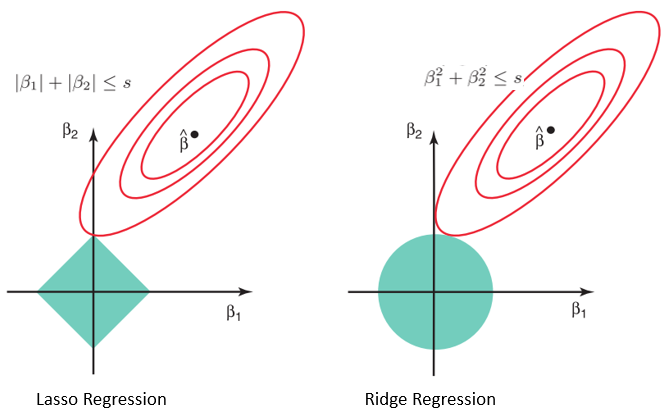
\includegraphics[width=1\linewidth]{fig/geo.png}
	\caption{Geometrijski prikaz $\ell^1$ in $\ell^2$ norme pri LASSO in Ridge regresiji v 2D prostoru parametrov modela.}
	\label{fig:vqvae}
\end{figure}

Na zgornji sliki je primerjava kaznovanja med LASSO in Ridge regresijo. Če enačbo za izračun paramterov v Lagrangeovi obliki zapišemo še za Ridge regresijo, takoj opazimo, da sta si problema na prvi pogled zelo podobna, vendar je razlika velika.

\begin{equation}
	\hat{\beta} =  \underset{\hat{\beta}}{\operatorname{argmin}} \{ ||y - X\beta||_2^2 + \lambda ||\beta||_2 \}
	\label{eqn5} 
\end{equation}

Kot je pokazano v enačbi \eqref{eqn5} pri Ridge regresiji prametre kaznujemo z $\ell^2$ normo. Če meje prikažemo v 2D prostoru parametrov modela, lahko vidimo, da je $\ell^2$ meja pri Ridge regresiji enaka $\beta_1^2 +\beta_2^2 \leq s$ in pri LASSO $|\beta_1| + |\beta_2| \leq s$, pri tem je $s$ stopnja kaznovanja. 

Opazimo, da bo površina, ki jo tvori $\beta_1^2 +\beta_2^2 \leq s$ meja Ridge regresije enaka krogu (v n-dimenzionalnemu prostoru n-krogla) in v primeru LASSO regresije ($|\beta_1| + |\beta_2| \leq s$) kvadrat, ki je rotiran tako, da oglišča ležijo na oseh (v večdimenzionalnem prostoru navzkrižni politop z oglišči na oseh). Ta detajl pokaže, kako LASSO določene parametre nastavi na natanko 0, medtem ko Ridge regresija ne, saj bo kontura parametrov zadela rob meje ravno v oglišču kvadrata (politopa), kar bo povzročilo, da bodo določeni parametri enaki točno 0, medtem ko bodo ostali zavzeli neko vrednost na osi.

\section*{Vrednost $\lambda$ in $t$}

Vrednost $\lambda$ v enačbi \eqref{eqn4} direktno nastavlja nivo krčenja (ang. shrinkage)




\end{document}

